\section{Normal SRP-PHAT vs MP-SRP-PHAT}
Comparison between the performance of normal SRP-PHAT vs MP-SRP-PHAT are done in this section. Simulations are provided to outline the robustness of the normal SRP-PHAT vs the MP-SRP-PHAT for various environmental aspects and sound source conditions. Effects of practical considerations such as the choice of array aperture size the recording sample rate, and the length of recording are shown. Finally, the robustness of the algorithms for errors in the microphone array placement are given.
\subsection{Effect of outdoor environment}
When localizing sound sources, the propagation environment can affect the signals received at the microphones. For outdoor environments, understanding the localization results thus requires knowledge of the physical phenomena at play at the time of the measurement\footnote{For more information on the theory behind outdoor sound propagation are refer Appendix \ref{app_outdoor}}. The effect of ground reflections, temperature and wind are provided here.
\subsubsection{Effect of ground reflections}
\begin{figure}[!ht]
\centering
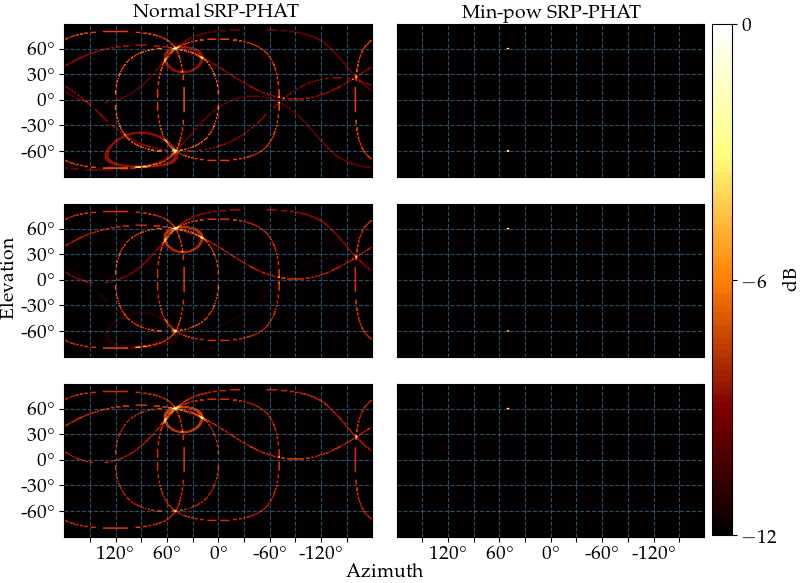
\includegraphics[width=\textwidth]{Figures/refSim.png}
\caption{Figures depict from top-to-bottom SRP-PHAT localization results for a source at ($50\degree$,$60\degree$) with ground reflection coefficients (R) of 1, 0.6 and 0.1. For normal SRP-PHAT, even though the image source should get significantly weaker for R=0.1, it does not as it is supported by the localization cones from the real source. MP-SRP-PHAT, however, is able to detect the source and the image powers correctly.}
\label{fig:4mic1srcRef}
\end{figure}
Sound received from a far-field sound source is the sum of a plane and a spherical wave component (Eq. \ref{Eq:GroundWave}). The spherical wave component creates a horizontal ground wave and quickly attenuates with distance. The plane wave component is reflected with the ground (image source), the magnitude of the reflection depends on the acoustic reflection coefficient of the ground material. Rudimentary simulations for a source located at $(\theta,\phi)$ can be made assuming image sound source located at $(\theta,-\phi)$. Fig. \ref{fig:4mic1srcRef} shows the localization results with a source at ($50\degree$,$60\degree$) for different ground reflection coefficients. The microphone pairs in the tetrahedral array that are parallel to the ground (horizontal) locate both the source and the image on the same cone. If the array is then placed such that three of its microphones are on the same horizontal plane, three out of the six possible cones will be shared. For normal SRP-PHAT, this causes the image to be localized at a higher level than it actually is\footnote{One way to mitigate this issue would be to not place the array horizontally, the simulations for this are given in Appendix \ref{sec:refTilted}}. 
\subsubsection{Effect of temperature}
\begin{figure}[!ht]
\centering
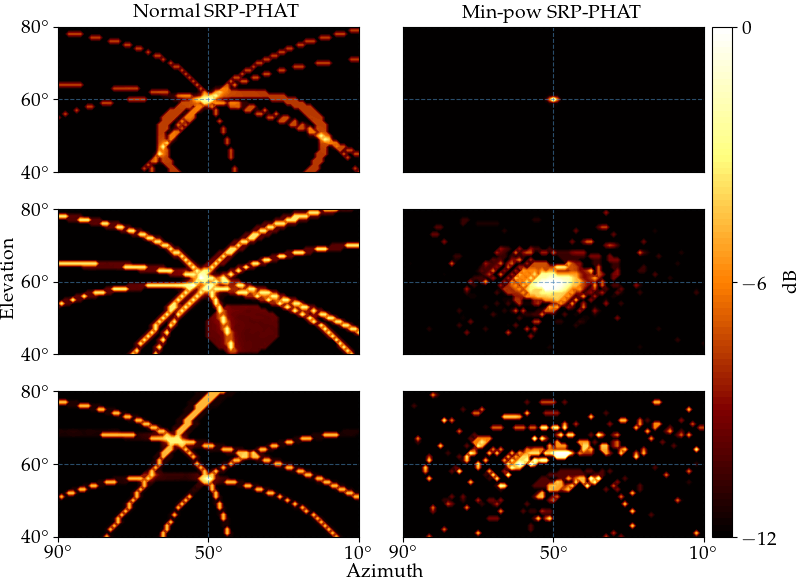
\includegraphics[width=\textwidth]{Figures/tempSim.png}
\caption{Figures depict from top-to-bottom SRP-PHAT localization results for a source at ($50\degree$,$60\degree$) with at temperatures of $20\degree C$, $0\degree C$ and $-40\degree C$. The extreme temperature of $-40\degree C$ is chosen to highlight the error.} 
\label{fig:4mic1srcTemp}
\end{figure}
Temperature affects the speed of sound and thus affects the delay time between the microphone pairs. During measurement, if the speed of sound is assumed to be 343m/sec, this could lead to errors in the localization results. Fig. \ref{fig:4mic1srcTemp} depicts the effect of temperature on localization results for a source at ($50\degree$,$60\degree$) , where wave files received by the tetrahedral microphone array at temperatures of $0\degree C$, $20\degree C$ and $-40\degree C$ are simulated. Then the localization is run assuming the speed of sound to be 343m/sec in every case. The figure shows zoomed in results around the source location. As can be seen in the figure, if temperature is not considered, it has the effect `de-focusing' the main peak. If temperature is recorded during measurements, the localization can be run using the correct speed of sound, which would remove this de-focusing issue\footnote{Since, the speed of sound is greater at higher temperatures, the number of samples that can fit within the array aperture would reduce. This can also have an effect on the localization results, however, this error is relatively minor. The effect of sample rates on localization results have been discussed later.}. For this reason, the temperature is recorded whenever outdoor measurements are done. 
\subsubsection{Effect of wind}
\begin{figure}[H]
\centering
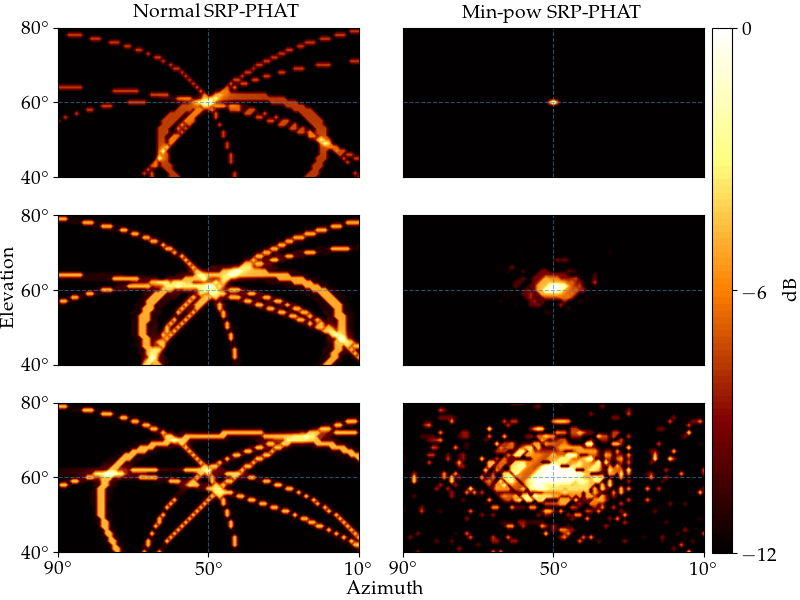
\includegraphics[width=\textwidth]{Figures/windSim.png}
\caption{Figures depict from top-to-bottom SRP-PHAT localization results with wind of $10 m/sec$ blowing $90\degree$, $10 m/sec$ blowing $45\degree$ and $30 m/sec$ blowing $45\degree$ to the source sound propagation direction. The extreme wind of $30 m/sec$ is chosen to highlight the error.}
\label{fig:4mic2srcWind}
\end{figure}
Wind speed effects the speed of sound in the direction of propagation. However unlike temperature, which causes a uniform difference in delays across the different microphone pairs, wind causes the delays to be affected differently depending on where the SRP search is looking and from what direction the wind is blowing. If wind blows perpendicular to the direction of propagation of the sound from the source, then it does not affect the localization. The maximum error happens exactly in and against the direction of the wind. Fig.\ref{fig:4mic2srcWind} depicts the effect of wind on localization results at wind of 10$m/s$ blowing at $90\degree$, $45\degree$ and $180\degree$ to the direction of propagation of sounds from a source at ($50\degree$,$60\degree$). It can be seen that when wind blows at $90\degree$, it does not affect the localization results. The magnitude of error when wind blows non-perpendicular to the sound propagation direction depends on the wind speed and the degree of alignment with the wind direction. For normal SRP-PHAT, an error in wind causes the localization cones to not overlap perfectly. For MP-SRP-PHAT, this causes a lowering of the peaks. This is because the localization circles are annular with peaks in the middle of the annular ring (a 3D torus). A movement in the tori causes the overlap to not happen perfectly, lowering the peaks. This error can be corrected during the SRP search, if the wind is recorded at the time of measurements. However, when doing outdoor measurements, the wind was rarely from a uniform direction. For this reason, the outdoor measurements were only done in relatively low wind conditions (<5m/sec), and no wind correction was applied.
\subsection{Effect of source conditions}
An extremely wide variety of outdoor sound sources exist. They can be spread-out or point sources, narrow-band or wide-band, be uniform across the frequency spectra, or have a lot of low frequency or high frequency content, moving or stationary, constant or transient. To keep the simulations within scope, some outdoor measurements were conducted to realize the major factors that can affect the localization. Based on those measurements, the effect of sound source SNR and the effect of coherence between multiple sound sources were selected. The simulations for those effects are given in this section.
\subsubsection{Effect of SNR}
\begin{figure}[H]
\centering
%\hspace*{-1cm}
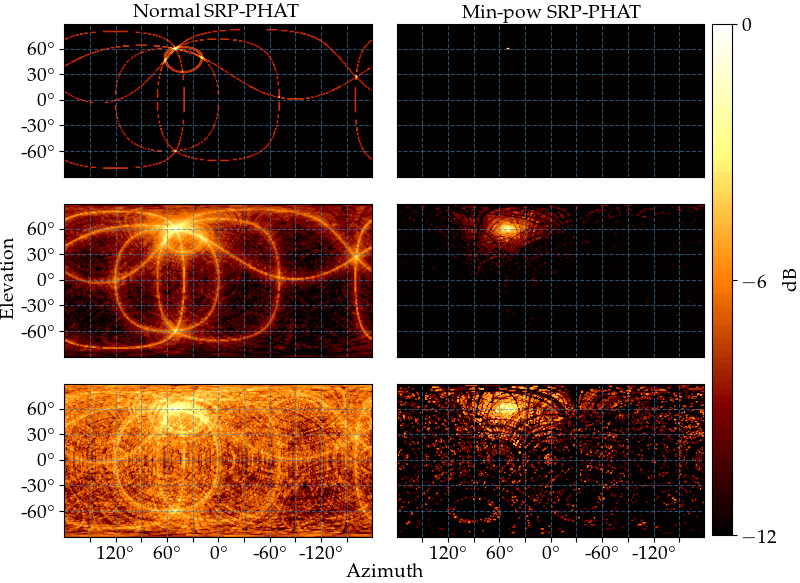
\includegraphics[width=\textwidth]{Figures/noiseSim.png}
\caption{Figures depict from top-to-bottom localization results with SNR = 20dB, SNR = 0dB, SNR = -6dB}
\label{fig:4mic1srcNoisy}
\end{figure}
The source SNR and overall magnitude is an important factor for localizing a source. Even if a source has a high sound level, if the SNR is low, the localization results might be poor. The error due to SNR has been discussed before for GCC comparison for a single pair of microphones, shown in Fig. \ref{fig:GCC_SIM}, where white noise is used for the simulations and it caused an almost uniform increase of the noise floor across all locations for GCC-PHAT. The same happens for tetrahedral localization, wherein, the noise floor across the entire noise map rises with falling SNR. Fig. \ref{fig:4mic1srcNoisy} shows the effect of source SNR on localization, with a point source at ($50\degree$, $60\degree$). As can be seen in the figure, the performance deteriorates as the SNR drops. However, understandably, the noise floor is lower for MP-SRP-PHAT, as it clears some of the noise results where not all cones overlap.
%\subsubsection{Minimum power SRP-PHAT}
\subsubsection{Effect of coherent sound sources}\label{sec:Coherent}\begin{figure}[H]
\centering
%\hspace*{-1cm}
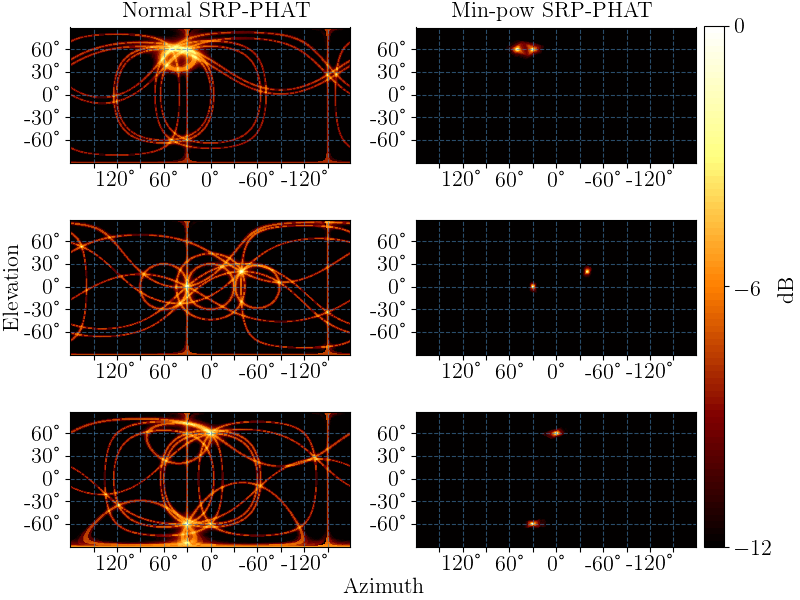
\includegraphics[width=\textwidth]{Figures/simCoherenceFalse.png}
\caption{Figures depict from top-to-bottom localization results for two sources located at ($50\degree$,$60\degree$) and ($30\degree$, $60\degree$), at ($40\degree$, $20\degree$) and ($30\degree$, $0\degree$), and at ($0\degree$, $60\degree$) and ($30\degree$, -$60\degree$) respectively. The sources are playing uncorrelated pink noise and the SNR is 6dB.}
\label{fig:4mic1srcCoherenceFalse}
\end{figure}
Fig. \ref{fig:4mic1srcCoherenceFalse} shows the localization results for two sound sources playing uncorrelated pink noise from different locations. As can be seen, both normal SRP-PHAT and MP-SRP-PHAT detect the peaks of the source correctly in all the cases. However, if multiple sound sources at different locations play coherently, i.e., the same waveform having a constant phase difference between each other, there is a possibility to detect a pseudo-source corresponding to the phase difference between the sound sources. This is because GCC algorithms inherently depend on the phase difference between the receiving waveforms to do the localization\footnote{The same error happens with human ears which causes detection of a stereo image in a 2 channel loudspeaker setup. Changing the inter-aural time difference causes this phantom image location to shift as well.}. The localization result for when 2 sources play the same pink noise are depicted in fig. \ref{fig:4mic1srcCoherence}. As can be seen in the figure, coherence has an effect on the localization, wherein, pseudo-peaks appear around the main sound source. The magnitude of these pseudo-peaks depends on their proximity and the phase difference. The effect of coherence is also seen later in an outdoor measurement, where multiple loudspeakers were playing music in an outdoor environment.
\begin{figure}[H]
\centering
%\hspace*{-1cm}
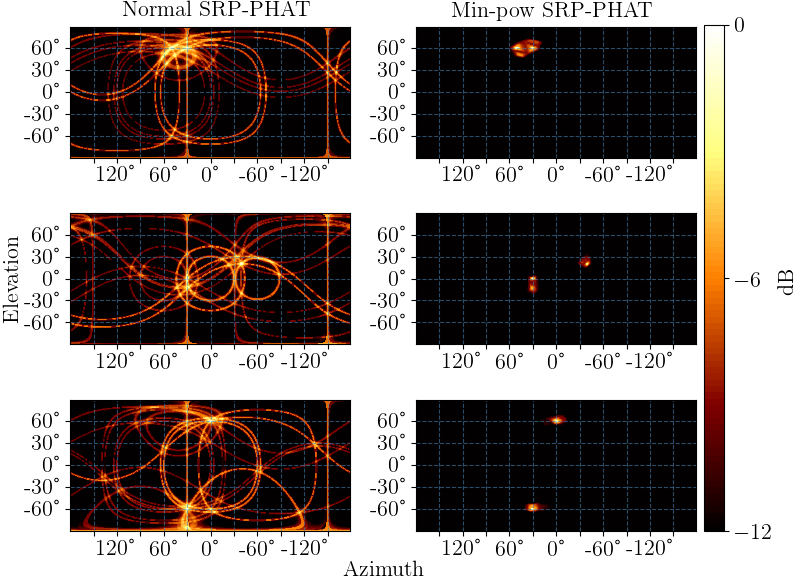
\includegraphics[width=\textwidth]{Figures/simCoherenceTrue.png}
\caption{Figures depict the localization results for when the sources from the previous figure play coherently. The sources here play the same pink noise. Pseudo-peaks can be seen to appear around the main sound sources.}
\label{fig:4mic1srcCoherence}
\end{figure}


